\documentclass[twoside]{book}

% Packages required by doxygen
\usepackage{fixltx2e}
\usepackage{calc}
\usepackage{doxygen}
\usepackage[export]{adjustbox} % also loads graphicx
\usepackage{graphicx}
\usepackage[utf8]{inputenc}
\usepackage{makeidx}
\usepackage{multicol}
\usepackage{multirow}
\PassOptionsToPackage{warn}{textcomp}
\usepackage{textcomp}
\usepackage[nointegrals]{wasysym}
\usepackage[table]{xcolor}

% Font selection
\usepackage[T1]{fontenc}
\usepackage[scaled=.90]{helvet}
\usepackage{courier}
\usepackage{amssymb}
\usepackage{sectsty}
\renewcommand{\familydefault}{\sfdefault}
\allsectionsfont{%
  \fontseries{bc}\selectfont%
  \color{darkgray}%
}
\renewcommand{\DoxyLabelFont}{%
  \fontseries{bc}\selectfont%
  \color{darkgray}%
}
\newcommand{\+}{\discretionary{\mbox{\scriptsize$\hookleftarrow$}}{}{}}

% Page & text layout
\usepackage{geometry}
\geometry{%
  a4paper,%
  top=2.5cm,%
  bottom=2.5cm,%
  left=2.5cm,%
  right=2.5cm%
}
\tolerance=750
\hfuzz=15pt
\hbadness=750
\setlength{\emergencystretch}{15pt}
\setlength{\parindent}{0cm}
\setlength{\parskip}{3ex plus 2ex minus 2ex}
\makeatletter
\renewcommand{\paragraph}{%
  \@startsection{paragraph}{4}{0ex}{-1.0ex}{1.0ex}{%
    \normalfont\normalsize\bfseries\SS@parafont%
  }%
}
\renewcommand{\subparagraph}{%
  \@startsection{subparagraph}{5}{0ex}{-1.0ex}{1.0ex}{%
    \normalfont\normalsize\bfseries\SS@subparafont%
  }%
}
\makeatother

% Headers & footers
\usepackage{fancyhdr}
\pagestyle{fancyplain}
\fancyhead[LE]{\fancyplain{}{\bfseries\thepage}}
\fancyhead[CE]{\fancyplain{}{}}
\fancyhead[RE]{\fancyplain{}{\bfseries\leftmark}}
\fancyhead[LO]{\fancyplain{}{\bfseries\rightmark}}
\fancyhead[CO]{\fancyplain{}{}}
\fancyhead[RO]{\fancyplain{}{\bfseries\thepage}}
\fancyfoot[LE]{\fancyplain{}{}}
\fancyfoot[CE]{\fancyplain{}{}}
\fancyfoot[RE]{\fancyplain{}{\bfseries\scriptsize Generated by Doxygen }}
\fancyfoot[LO]{\fancyplain{}{\bfseries\scriptsize Generated by Doxygen }}
\fancyfoot[CO]{\fancyplain{}{}}
\fancyfoot[RO]{\fancyplain{}{}}
\renewcommand{\footrulewidth}{0.4pt}
\renewcommand{\chaptermark}[1]{%
  \markboth{#1}{}%
}
\renewcommand{\sectionmark}[1]{%
  \markright{\thesection\ #1}%
}

% Indices & bibliography
\usepackage{natbib}
\usepackage[titles]{tocloft}
\setcounter{tocdepth}{3}
\setcounter{secnumdepth}{5}
\makeindex

% Hyperlinks (required, but should be loaded last)
\usepackage{ifpdf}
\ifpdf
  \usepackage[pdftex,pagebackref=true]{hyperref}
\else
  \usepackage[ps2pdf,pagebackref=true]{hyperref}
\fi
\hypersetup{%
  colorlinks=true,%
  linkcolor=blue,%
  citecolor=blue,%
  unicode%
}

% Custom commands
\newcommand{\clearemptydoublepage}{%
  \newpage{\pagestyle{empty}\cleardoublepage}%
}

\usepackage{caption}
\captionsetup{labelsep=space,justification=centering,font={bf},singlelinecheck=off,skip=4pt,position=top}

%===== C O N T E N T S =====

\begin{document}

% Titlepage & ToC
\hypersetup{pageanchor=false,
             bookmarksnumbered=true,
             pdfencoding=unicode
            }
\pagenumbering{roman}
\begin{titlepage}
\vspace*{7cm}
\begin{center}%
{\Large Armagetron\+Server }\\
\vspace*{1cm}
{\large Generated by Doxygen 1.8.11}\\
\end{center}
\end{titlepage}
\clearemptydoublepage
\tableofcontents
\clearemptydoublepage
\pagenumbering{arabic}
\hypersetup{pageanchor=true}

%--- Begin generated contents ---
\chapter{L\+I\+C\+E\+N\+SE}
\label{md_D:_owncloud_HEIG-VD_JavaProjects_GEN_Armagetron_Serveur_LICENSE}
\hypertarget{md_D:_owncloud_HEIG-VD_JavaProjects_GEN_Armagetron_Serveur_LICENSE}{}
\input{md_D:_owncloud_HEIG-VD_JavaProjects_GEN_Armagetron_Serveur_LICENSE}
\chapter{Namespace Index}
\section{Packages}
Here are the packages with brief descriptions (if available)\+:\begin{DoxyCompactList}
\item\contentsline{section}{\hyperlink{namespaceclient_test}{client\+Test} }{\pageref{namespaceclient_test}}{}
\item\contentsline{section}{\hyperlink{namespaceserver}{server} }{\pageref{namespaceserver}}{}
\end{DoxyCompactList}

\chapter{Hierarchical Index}
\section{Class Hierarchy}
This inheritance list is sorted roughly, but not completely, alphabetically\+:\begin{DoxyCompactList}
\item \contentsline{section}{server.\+Box\+Test}{\pageref{classserver_1_1_box_test}}{}
\item \contentsline{section}{server.\+Controller\+Test}{\pageref{classserver_1_1_controller_test}}{}
\item \contentsline{section}{server.\+Game\+Test}{\pageref{classserver_1_1_game_test}}{}
\item \contentsline{section}{server.\+Location}{\pageref{classserver_1_1_location}}{}
\item \contentsline{section}{server.\+Main}{\pageref{classserver_1_1_main}}{}
\item Runnable\begin{DoxyCompactList}
\item \contentsline{section}{client\+Test.\+Client}{\pageref{classclient_test_1_1_client}}{}
\item \contentsline{section}{server.\+Server}{\pageref{classserver_1_1_server}}{}
\end{DoxyCompactList}
\item \contentsline{section}{server.\+Serveur\+Tests}{\pageref{classserver_1_1_serveur_tests}}{}
\end{DoxyCompactList}

\chapter{Class Index}
\section{Class List}
Here are the classes, structs, unions and interfaces with brief descriptions\+:\begin{DoxyCompactList}
\item\contentsline{section}{\hyperlink{classserver_1_1_box_test}{server.\+Box\+Test} }{\pageref{classserver_1_1_box_test}}{}
\item\contentsline{section}{\hyperlink{classclient_test_1_1_client}{client\+Test.\+Client} }{\pageref{classclient_test_1_1_client}}{}
\item\contentsline{section}{\hyperlink{classserver_1_1_controller_test}{server.\+Controller\+Test} }{\pageref{classserver_1_1_controller_test}}{}
\item\contentsline{section}{\hyperlink{classserver_1_1_game_test}{server.\+Game\+Test} }{\pageref{classserver_1_1_game_test}}{}
\item\contentsline{section}{\hyperlink{classserver_1_1_location}{server.\+Location} }{\pageref{classserver_1_1_location}}{}
\item\contentsline{section}{\hyperlink{classserver_1_1_main}{server.\+Main} }{\pageref{classserver_1_1_main}}{}
\item\contentsline{section}{\hyperlink{classserver_1_1_server}{server.\+Server} }{\pageref{classserver_1_1_server}}{}
\item\contentsline{section}{\hyperlink{classserver_1_1_serveur_tests}{server.\+Serveur\+Tests} }{\pageref{classserver_1_1_serveur_tests}}{}
\end{DoxyCompactList}

\chapter{File Index}
\section{File List}
Here is a list of all files with brief descriptions\+:\begin{DoxyCompactList}
\item\contentsline{section}{D\+:/owncloud/\+H\+E\+I\+G-\/\+V\+D/\+Java\+Projects/\+G\+E\+N\+\_\+\+Armagetron\+\_\+\+Serveur/src/main/java/client\+Test/\hyperlink{_client_8java}{Client.\+java} }{\pageref{_client_8java}}{}
\item\contentsline{section}{D\+:/owncloud/\+H\+E\+I\+G-\/\+V\+D/\+Java\+Projects/\+G\+E\+N\+\_\+\+Armagetron\+\_\+\+Serveur/src/main/java/server/\hyperlink{_box_8java}{Box.\+java} \\*\+: Class Box contained in the Grid\+Game }{\pageref{_box_8java}}{}
\item\contentsline{section}{D\+:/owncloud/\+H\+E\+I\+G-\/\+V\+D/\+Java\+Projects/\+G\+E\+N\+\_\+\+Armagetron\+\_\+\+Serveur/src/main/java/server/\hyperlink{_client_thread_8java}{Client\+Thread.\+java} \\*\+: Use as interface between client and controller to receive object from server, send object to server and connect to the server }{\pageref{_client_thread_8java}}{}
\item\contentsline{section}{D\+:/owncloud/\+H\+E\+I\+G-\/\+V\+D/\+Java\+Projects/\+G\+E\+N\+\_\+\+Armagetron\+\_\+\+Serveur/src/main/java/server/\hyperlink{_controller_8java}{Controller.\+java} \\*\+: Check all data between Game and Server }{\pageref{_controller_8java}}{}
\item\contentsline{section}{D\+:/owncloud/\+H\+E\+I\+G-\/\+V\+D/\+Java\+Projects/\+G\+E\+N\+\_\+\+Armagetron\+\_\+\+Serveur/src/main/java/server/\hyperlink{_game_8java}{Game.\+java} \\*\+: Use only for the Tests }{\pageref{_game_8java}}{}
\item\contentsline{section}{D\+:/owncloud/\+H\+E\+I\+G-\/\+V\+D/\+Java\+Projects/\+G\+E\+N\+\_\+\+Armagetron\+\_\+\+Serveur/src/main/java/server/\hyperlink{_game_grid_8java}{Game\+Grid.\+java} \\*\+: class use to manage the Game\+Grid }{\pageref{_game_grid_8java}}{}
\item\contentsline{section}{D\+:/owncloud/\+H\+E\+I\+G-\/\+V\+D/\+Java\+Projects/\+G\+E\+N\+\_\+\+Armagetron\+\_\+\+Serveur/src/main/java/server/\hyperlink{_location_8java}{Location.\+java} \\*\+: Class Location use to set Starting location to player }{\pageref{_location_8java}}{}
\item\contentsline{section}{D\+:/owncloud/\+H\+E\+I\+G-\/\+V\+D/\+Java\+Projects/\+G\+E\+N\+\_\+\+Armagetron\+\_\+\+Serveur/src/main/java/server/\hyperlink{_main_8java}{Main.\+java} \\*\+: Start a new server }{\pageref{_main_8java}}{}
\item\contentsline{section}{D\+:/owncloud/\+H\+E\+I\+G-\/\+V\+D/\+Java\+Projects/\+G\+E\+N\+\_\+\+Armagetron\+\_\+\+Serveur/src/main/java/server/\hyperlink{_player_8java}{Player.\+java} \\*\+: Use to manage a player }{\pageref{_player_8java}}{}
\item\contentsline{section}{D\+:/owncloud/\+H\+E\+I\+G-\/\+V\+D/\+Java\+Projects/\+G\+E\+N\+\_\+\+Armagetron\+\_\+\+Serveur/src/main/java/server/\hyperlink{_server_8java}{Server.\+java} \\*\+: Server }{\pageref{_server_8java}}{}
\item\contentsline{section}{D\+:/owncloud/\+H\+E\+I\+G-\/\+V\+D/\+Java\+Projects/\+G\+E\+N\+\_\+\+Armagetron\+\_\+\+Serveur/src/test/java/server/\hyperlink{_box_test_8java}{Box\+Test.\+java} \\*\+: Test the class Box }{\pageref{_box_test_8java}}{}
\item\contentsline{section}{D\+:/owncloud/\+H\+E\+I\+G-\/\+V\+D/\+Java\+Projects/\+G\+E\+N\+\_\+\+Armagetron\+\_\+\+Serveur/src/test/java/server/\hyperlink{_controller_test_8java}{Controller\+Test.\+java} \\*\+: Test the class Controller\+Test }{\pageref{_controller_test_8java}}{}
\item\contentsline{section}{D\+:/owncloud/\+H\+E\+I\+G-\/\+V\+D/\+Java\+Projects/\+G\+E\+N\+\_\+\+Armagetron\+\_\+\+Serveur/src/test/java/server/\hyperlink{_game_test_8java}{Game\+Test.\+java} }{\pageref{_game_test_8java}}{}
\item\contentsline{section}{D\+:/owncloud/\+H\+E\+I\+G-\/\+V\+D/\+Java\+Projects/\+G\+E\+N\+\_\+\+Armagetron\+\_\+\+Serveur/src/test/java/server/\hyperlink{_serveur_tests_8java}{Serveur\+Tests.\+java} \\*\+: Class vérifiant les collisions sur le serveur }{\pageref{_serveur_tests_8java}}{}
\item\contentsline{section}{D\+:/owncloud/\+H\+E\+I\+G-\/\+V\+D/\+Java\+Projects/\+G\+E\+N\+\_\+\+Armagetron\+\_\+\+Serveur/src/test/java/server/\hyperlink{_test_utils_8java}{Test\+Utils.\+java} \\*\+: Utils Object shared by Test class }{\pageref{_test_utils_8java}}{}
\end{DoxyCompactList}

\chapter{Namespace Documentation}
\hypertarget{namespaceclient_test}{}\section{Package client\+Test}
\label{namespaceclient_test}\index{client\+Test@{client\+Test}}
\subsection*{Classes}
\begin{DoxyCompactItemize}
\item 
class \hyperlink{classclient_test_1_1_client}{Client}
\end{DoxyCompactItemize}

\hypertarget{namespaceserver}{}\section{Package server}
\label{namespaceserver}\index{server@{server}}
\subsection*{Classes}
\begin{DoxyCompactItemize}
\item 
class {\bfseries Box}
\item 
class \hyperlink{classserver_1_1_box_test}{Box\+Test}
\item 
class {\bfseries Client\+Thread}
\item 
class {\bfseries Controller}
\item 
class \hyperlink{classserver_1_1_controller_test}{Controller\+Test}
\item 
class {\bfseries Game}
\item 
class {\bfseries Game\+Grid}
\item 
class \hyperlink{classserver_1_1_game_test}{Game\+Test}
\item 
class \hyperlink{classserver_1_1_location}{Location}
\item 
class \hyperlink{classserver_1_1_main}{Main}
\item 
class {\bfseries Player}
\item 
class \hyperlink{classserver_1_1_server}{Server}
\item 
class \hyperlink{classserver_1_1_serveur_tests}{Serveur\+Tests}
\item 
class {\bfseries Test\+Utils}
\end{DoxyCompactItemize}

\chapter{Class Documentation}
\hypertarget{classserver_1_1_box_test}{}\section{server.\+Box\+Test Class Reference}
\label{classserver_1_1_box_test}\index{server.\+Box\+Test@{server.\+Box\+Test}}
\subsection*{Public Member Functions}
\begin{DoxyCompactItemize}
\item 
void \hyperlink{classserver_1_1_box_test_a11a1f3f1f7c7506ad14b9ac4053a25db}{get\+Set\+Color} ()  throws Exception 
\item 
void \hyperlink{classserver_1_1_box_test_abff1f031ff833649d8558f036cfc17f7}{get\+Set\+Id} ()  throws Exception 
\item 
void \hyperlink{classserver_1_1_box_test_a2965a10a30ad8d24501e5144801983e3}{is\+Empty} ()  throws Exception 
\item 
void \hyperlink{classserver_1_1_box_test_ae5f4f7940e892d55f69025c818533fe4}{can\+Create\+Box} ()  throws Exception 
\end{DoxyCompactItemize}


\subsection{Detailed Description}


Definition at line 18 of file Box\+Test.\+java.



\subsection{Member Function Documentation}
\index{server\+::\+Box\+Test@{server\+::\+Box\+Test}!can\+Create\+Box@{can\+Create\+Box}}
\index{can\+Create\+Box@{can\+Create\+Box}!server\+::\+Box\+Test@{server\+::\+Box\+Test}}
\subsubsection[{\texorpdfstring{can\+Create\+Box()}{canCreateBox()}}]{\setlength{\rightskip}{0pt plus 5cm}void server.\+Box\+Test.\+can\+Create\+Box (
\begin{DoxyParamCaption}
{}
\end{DoxyParamCaption}
) throws Exception}\hypertarget{classserver_1_1_box_test_ae5f4f7940e892d55f69025c818533fe4}{}\label{classserver_1_1_box_test_ae5f4f7940e892d55f69025c818533fe4}


Definition at line 50 of file Box\+Test.\+java.

\index{server\+::\+Box\+Test@{server\+::\+Box\+Test}!get\+Set\+Color@{get\+Set\+Color}}
\index{get\+Set\+Color@{get\+Set\+Color}!server\+::\+Box\+Test@{server\+::\+Box\+Test}}
\subsubsection[{\texorpdfstring{get\+Set\+Color()}{getSetColor()}}]{\setlength{\rightskip}{0pt plus 5cm}void server.\+Box\+Test.\+get\+Set\+Color (
\begin{DoxyParamCaption}
{}
\end{DoxyParamCaption}
) throws Exception}\hypertarget{classserver_1_1_box_test_a11a1f3f1f7c7506ad14b9ac4053a25db}{}\label{classserver_1_1_box_test_a11a1f3f1f7c7506ad14b9ac4053a25db}


Definition at line 21 of file Box\+Test.\+java.

\index{server\+::\+Box\+Test@{server\+::\+Box\+Test}!get\+Set\+Id@{get\+Set\+Id}}
\index{get\+Set\+Id@{get\+Set\+Id}!server\+::\+Box\+Test@{server\+::\+Box\+Test}}
\subsubsection[{\texorpdfstring{get\+Set\+Id()}{getSetId()}}]{\setlength{\rightskip}{0pt plus 5cm}void server.\+Box\+Test.\+get\+Set\+Id (
\begin{DoxyParamCaption}
{}
\end{DoxyParamCaption}
) throws Exception}\hypertarget{classserver_1_1_box_test_abff1f031ff833649d8558f036cfc17f7}{}\label{classserver_1_1_box_test_abff1f031ff833649d8558f036cfc17f7}


Definition at line 32 of file Box\+Test.\+java.

\index{server\+::\+Box\+Test@{server\+::\+Box\+Test}!is\+Empty@{is\+Empty}}
\index{is\+Empty@{is\+Empty}!server\+::\+Box\+Test@{server\+::\+Box\+Test}}
\subsubsection[{\texorpdfstring{is\+Empty()}{isEmpty()}}]{\setlength{\rightskip}{0pt plus 5cm}void server.\+Box\+Test.\+is\+Empty (
\begin{DoxyParamCaption}
{}
\end{DoxyParamCaption}
) throws Exception}\hypertarget{classserver_1_1_box_test_a2965a10a30ad8d24501e5144801983e3}{}\label{classserver_1_1_box_test_a2965a10a30ad8d24501e5144801983e3}


Definition at line 43 of file Box\+Test.\+java.



The documentation for this class was generated from the following file\+:\begin{DoxyCompactItemize}
\item 
D\+:/owncloud/\+H\+E\+I\+G-\/\+V\+D/\+Java\+Projects/\+G\+E\+N\+\_\+\+Armagetron\+\_\+\+Serveur/src/test/java/server/\hyperlink{_box_test_8java}{Box\+Test.\+java}\end{DoxyCompactItemize}

\hypertarget{classclient_test_1_1_client}{}\section{client\+Test.\+Client Class Reference}
\label{classclient_test_1_1_client}\index{client\+Test.\+Client@{client\+Test.\+Client}}
Inheritance diagram for client\+Test.\+Client\+:\begin{figure}[H]
\begin{center}
\leavevmode
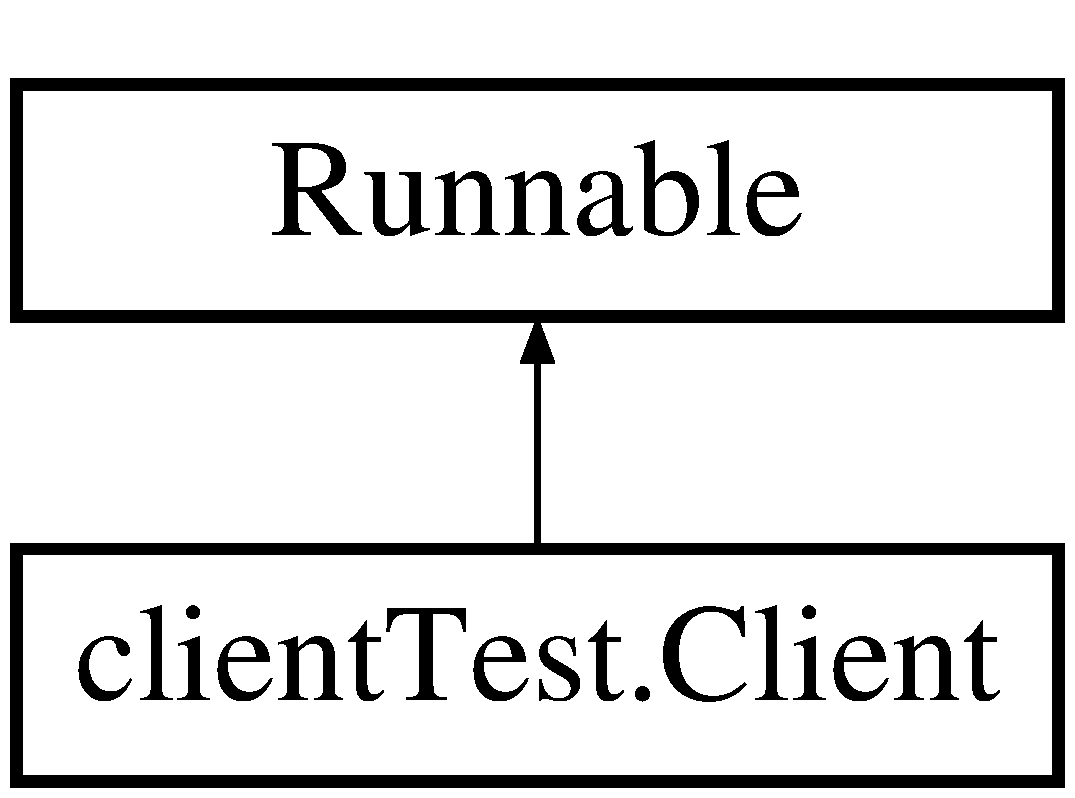
\includegraphics[height=2.000000cm]{classclient_test_1_1_client}
\end{center}
\end{figure}
\subsection*{Public Member Functions}
\begin{DoxyCompactItemize}
\item 
\hyperlink{classclient_test_1_1_client_a4f9854e466dd46a4d781f8f09ca03100}{Client} (String server\+Address, int port)
\item 
void \hyperlink{classclient_test_1_1_client_a64a94429877c2bc46115cf9427044551}{run} ()
\begin{DoxyCompactList}\small\item\em Listen to receive object from the server. \end{DoxyCompactList}\end{DoxyCompactItemize}


\subsection{Detailed Description}


Definition at line 25 of file Client.\+java.



\subsection{Constructor \& Destructor Documentation}
\index{client\+Test\+::\+Client@{client\+Test\+::\+Client}!Client@{Client}}
\index{Client@{Client}!client\+Test\+::\+Client@{client\+Test\+::\+Client}}
\subsubsection[{\texorpdfstring{Client(\+String server\+Address, int port)}{Client(String serverAddress, int port)}}]{\setlength{\rightskip}{0pt plus 5cm}client\+Test.\+Client.\+Client (
\begin{DoxyParamCaption}
\item[{String}]{server\+Address, }
\item[{int}]{port}
\end{DoxyParamCaption}
)}\hypertarget{classclient_test_1_1_client_a4f9854e466dd46a4d781f8f09ca03100}{}\label{classclient_test_1_1_client_a4f9854e466dd46a4d781f8f09ca03100}
Constructor


\begin{DoxyParams}{Parameters}
{\em server\+Address} & The server Adress \\
\hline
{\em port} & The server\textquotesingle{}s port \\
\hline
\end{DoxyParams}


Definition at line 42 of file Client.\+java.



\subsection{Member Function Documentation}
\index{client\+Test\+::\+Client@{client\+Test\+::\+Client}!run@{run}}
\index{run@{run}!client\+Test\+::\+Client@{client\+Test\+::\+Client}}
\subsubsection[{\texorpdfstring{run()}{run()}}]{\setlength{\rightskip}{0pt plus 5cm}public void client\+Test.\+Client.\+run (
\begin{DoxyParamCaption}
{}
\end{DoxyParamCaption}
)}\hypertarget{classclient_test_1_1_client_a64a94429877c2bc46115cf9427044551}{}\label{classclient_test_1_1_client_a64a94429877c2bc46115cf9427044551}


Listen to receive object from the server. 

\begin{DoxyAuthor}{Author}
Michael Brouchoud 
\end{DoxyAuthor}


Definition at line 147 of file Client.\+java.



The documentation for this class was generated from the following file\+:\begin{DoxyCompactItemize}
\item 
D\+:/owncloud/\+H\+E\+I\+G-\/\+V\+D/\+Java\+Projects/\+G\+E\+N\+\_\+\+Armagetron\+\_\+\+Serveur/src/main/java/client\+Test/\hyperlink{_client_8java}{Client.\+java}\end{DoxyCompactItemize}

\hypertarget{classserver_1_1_controller_test}{}\section{server.\+Controller\+Test Class Reference}
\label{classserver_1_1_controller_test}\index{server.\+Controller\+Test@{server.\+Controller\+Test}}
\subsection*{Public Member Functions}
\begin{DoxyCompactItemize}
\item 
void \hyperlink{classserver_1_1_controller_test_a3da69db9b77369d656fc7a7ab10aa51d}{before\+Start} ()
\item 
void \hyperlink{classserver_1_1_controller_test_a698e419a47a1e7028c75c0fc41ee632a}{start\+Game} ()  throws Exception 
\item 
void \hyperlink{classserver_1_1_controller_test_ac869ba0e796f883075610a615bbda101}{end\+Game} ()  throws Exception 
\item 
void \hyperlink{classserver_1_1_controller_test_ae90961ba9a964626b10a7225a6bd09ec}{process\+Data} ()  throws Exception 
\item 
void \hyperlink{classserver_1_1_controller_test_ae1119bb8a1bab8895006daa4bb661ae3}{send\+Game} ()  throws Exception 
\item 
void \hyperlink{classserver_1_1_controller_test_ad326704657c09a31a13615b9d49bf396}{can\+Create\+Controller} ()  throws Exception 
\end{DoxyCompactItemize}


\subsection{Detailed Description}


Definition at line 21 of file Controller\+Test.\+java.



\subsection{Member Function Documentation}
\index{server\+::\+Controller\+Test@{server\+::\+Controller\+Test}!before\+Start@{before\+Start}}
\index{before\+Start@{before\+Start}!server\+::\+Controller\+Test@{server\+::\+Controller\+Test}}
\subsubsection[{\texorpdfstring{before\+Start()}{beforeStart()}}]{\setlength{\rightskip}{0pt plus 5cm}void server.\+Controller\+Test.\+before\+Start (
\begin{DoxyParamCaption}
{}
\end{DoxyParamCaption}
)}\hypertarget{classserver_1_1_controller_test_a3da69db9b77369d656fc7a7ab10aa51d}{}\label{classserver_1_1_controller_test_a3da69db9b77369d656fc7a7ab10aa51d}


Definition at line 25 of file Controller\+Test.\+java.

\index{server\+::\+Controller\+Test@{server\+::\+Controller\+Test}!can\+Create\+Controller@{can\+Create\+Controller}}
\index{can\+Create\+Controller@{can\+Create\+Controller}!server\+::\+Controller\+Test@{server\+::\+Controller\+Test}}
\subsubsection[{\texorpdfstring{can\+Create\+Controller()}{canCreateController()}}]{\setlength{\rightskip}{0pt plus 5cm}void server.\+Controller\+Test.\+can\+Create\+Controller (
\begin{DoxyParamCaption}
{}
\end{DoxyParamCaption}
) throws Exception}\hypertarget{classserver_1_1_controller_test_ad326704657c09a31a13615b9d49bf396}{}\label{classserver_1_1_controller_test_ad326704657c09a31a13615b9d49bf396}


Definition at line 74 of file Controller\+Test.\+java.

\index{server\+::\+Controller\+Test@{server\+::\+Controller\+Test}!end\+Game@{end\+Game}}
\index{end\+Game@{end\+Game}!server\+::\+Controller\+Test@{server\+::\+Controller\+Test}}
\subsubsection[{\texorpdfstring{end\+Game()}{endGame()}}]{\setlength{\rightskip}{0pt plus 5cm}void server.\+Controller\+Test.\+end\+Game (
\begin{DoxyParamCaption}
{}
\end{DoxyParamCaption}
) throws Exception}\hypertarget{classserver_1_1_controller_test_ac869ba0e796f883075610a615bbda101}{}\label{classserver_1_1_controller_test_ac869ba0e796f883075610a615bbda101}


Definition at line 39 of file Controller\+Test.\+java.

\index{server\+::\+Controller\+Test@{server\+::\+Controller\+Test}!process\+Data@{process\+Data}}
\index{process\+Data@{process\+Data}!server\+::\+Controller\+Test@{server\+::\+Controller\+Test}}
\subsubsection[{\texorpdfstring{process\+Data()}{processData()}}]{\setlength{\rightskip}{0pt plus 5cm}void server.\+Controller\+Test.\+process\+Data (
\begin{DoxyParamCaption}
{}
\end{DoxyParamCaption}
) throws Exception}\hypertarget{classserver_1_1_controller_test_ae90961ba9a964626b10a7225a6bd09ec}{}\label{classserver_1_1_controller_test_ae90961ba9a964626b10a7225a6bd09ec}


Definition at line 50 of file Controller\+Test.\+java.

\index{server\+::\+Controller\+Test@{server\+::\+Controller\+Test}!send\+Game@{send\+Game}}
\index{send\+Game@{send\+Game}!server\+::\+Controller\+Test@{server\+::\+Controller\+Test}}
\subsubsection[{\texorpdfstring{send\+Game()}{sendGame()}}]{\setlength{\rightskip}{0pt plus 5cm}void server.\+Controller\+Test.\+send\+Game (
\begin{DoxyParamCaption}
{}
\end{DoxyParamCaption}
) throws Exception}\hypertarget{classserver_1_1_controller_test_ae1119bb8a1bab8895006daa4bb661ae3}{}\label{classserver_1_1_controller_test_ae1119bb8a1bab8895006daa4bb661ae3}


Definition at line 62 of file Controller\+Test.\+java.

\index{server\+::\+Controller\+Test@{server\+::\+Controller\+Test}!start\+Game@{start\+Game}}
\index{start\+Game@{start\+Game}!server\+::\+Controller\+Test@{server\+::\+Controller\+Test}}
\subsubsection[{\texorpdfstring{start\+Game()}{startGame()}}]{\setlength{\rightskip}{0pt plus 5cm}void server.\+Controller\+Test.\+start\+Game (
\begin{DoxyParamCaption}
{}
\end{DoxyParamCaption}
) throws Exception}\hypertarget{classserver_1_1_controller_test_a698e419a47a1e7028c75c0fc41ee632a}{}\label{classserver_1_1_controller_test_a698e419a47a1e7028c75c0fc41ee632a}


Definition at line 34 of file Controller\+Test.\+java.



The documentation for this class was generated from the following file\+:\begin{DoxyCompactItemize}
\item 
D\+:/owncloud/\+H\+E\+I\+G-\/\+V\+D/\+Java\+Projects/\+G\+E\+N\+\_\+\+Armagetron\+\_\+\+Serveur/src/test/java/server/\hyperlink{_controller_test_8java}{Controller\+Test.\+java}\end{DoxyCompactItemize}

\hypertarget{classserver_1_1_game_test}{}\section{server.\+Game\+Test Class Reference}
\label{classserver_1_1_game_test}\index{server.\+Game\+Test@{server.\+Game\+Test}}
\subsection*{Public Member Functions}
\begin{DoxyCompactItemize}
\item 
void \hyperlink{classserver_1_1_game_test_aba104902743134d29154f865a6972c1e}{add} ()  throws Exception 
\item 
void \hyperlink{classserver_1_1_game_test_a93938db84ab5a7ce1ea2c01793ecce85}{get\+Players} ()  throws Exception 
\item 
void \hyperlink{classserver_1_1_game_test_a163ba477ae389481b94311b53ba478e6}{get\+Player} ()  throws Exception 
\item 
void \hyperlink{classserver_1_1_game_test_a638136da6a27b8f4845943f86c8d8057}{start\+Stopis\+Running} ()  throws Exception 
\item 
void \hyperlink{classserver_1_1_game_test_a835dc5fe6c5462a0cc889a222632055d}{can\+Create\+Game} ()  throws Exception 
\end{DoxyCompactItemize}


\subsection{Detailed Description}


Definition at line 7 of file Game\+Test.\+java.



\subsection{Member Function Documentation}
\index{server\+::\+Game\+Test@{server\+::\+Game\+Test}!add@{add}}
\index{add@{add}!server\+::\+Game\+Test@{server\+::\+Game\+Test}}
\subsubsection[{\texorpdfstring{add()}{add()}}]{\setlength{\rightskip}{0pt plus 5cm}void server.\+Game\+Test.\+add (
\begin{DoxyParamCaption}
{}
\end{DoxyParamCaption}
) throws Exception}\hypertarget{classserver_1_1_game_test_aba104902743134d29154f865a6972c1e}{}\label{classserver_1_1_game_test_aba104902743134d29154f865a6972c1e}


Definition at line 9 of file Game\+Test.\+java.

\index{server\+::\+Game\+Test@{server\+::\+Game\+Test}!can\+Create\+Game@{can\+Create\+Game}}
\index{can\+Create\+Game@{can\+Create\+Game}!server\+::\+Game\+Test@{server\+::\+Game\+Test}}
\subsubsection[{\texorpdfstring{can\+Create\+Game()}{canCreateGame()}}]{\setlength{\rightskip}{0pt plus 5cm}void server.\+Game\+Test.\+can\+Create\+Game (
\begin{DoxyParamCaption}
{}
\end{DoxyParamCaption}
) throws Exception}\hypertarget{classserver_1_1_game_test_a835dc5fe6c5462a0cc889a222632055d}{}\label{classserver_1_1_game_test_a835dc5fe6c5462a0cc889a222632055d}


Definition at line 55 of file Game\+Test.\+java.

\index{server\+::\+Game\+Test@{server\+::\+Game\+Test}!get\+Player@{get\+Player}}
\index{get\+Player@{get\+Player}!server\+::\+Game\+Test@{server\+::\+Game\+Test}}
\subsubsection[{\texorpdfstring{get\+Player()}{getPlayer()}}]{\setlength{\rightskip}{0pt plus 5cm}void server.\+Game\+Test.\+get\+Player (
\begin{DoxyParamCaption}
{}
\end{DoxyParamCaption}
) throws Exception}\hypertarget{classserver_1_1_game_test_a163ba477ae389481b94311b53ba478e6}{}\label{classserver_1_1_game_test_a163ba477ae389481b94311b53ba478e6}


Definition at line 29 of file Game\+Test.\+java.

\index{server\+::\+Game\+Test@{server\+::\+Game\+Test}!get\+Players@{get\+Players}}
\index{get\+Players@{get\+Players}!server\+::\+Game\+Test@{server\+::\+Game\+Test}}
\subsubsection[{\texorpdfstring{get\+Players()}{getPlayers()}}]{\setlength{\rightskip}{0pt plus 5cm}void server.\+Game\+Test.\+get\+Players (
\begin{DoxyParamCaption}
{}
\end{DoxyParamCaption}
) throws Exception}\hypertarget{classserver_1_1_game_test_a93938db84ab5a7ce1ea2c01793ecce85}{}\label{classserver_1_1_game_test_a93938db84ab5a7ce1ea2c01793ecce85}


Definition at line 23 of file Game\+Test.\+java.

\index{server\+::\+Game\+Test@{server\+::\+Game\+Test}!start\+Stopis\+Running@{start\+Stopis\+Running}}
\index{start\+Stopis\+Running@{start\+Stopis\+Running}!server\+::\+Game\+Test@{server\+::\+Game\+Test}}
\subsubsection[{\texorpdfstring{start\+Stopis\+Running()}{startStopisRunning()}}]{\setlength{\rightskip}{0pt plus 5cm}void server.\+Game\+Test.\+start\+Stopis\+Running (
\begin{DoxyParamCaption}
{}
\end{DoxyParamCaption}
) throws Exception}\hypertarget{classserver_1_1_game_test_a638136da6a27b8f4845943f86c8d8057}{}\label{classserver_1_1_game_test_a638136da6a27b8f4845943f86c8d8057}


Definition at line 41 of file Game\+Test.\+java.



The documentation for this class was generated from the following file\+:\begin{DoxyCompactItemize}
\item 
D\+:/owncloud/\+H\+E\+I\+G-\/\+V\+D/\+Java\+Projects/\+G\+E\+N\+\_\+\+Armagetron\+\_\+\+Serveur/src/test/java/server/\hyperlink{_game_test_8java}{Game\+Test.\+java}\end{DoxyCompactItemize}

\hypertarget{classserver_1_1_location}{}\section{server.\+Location Class Reference}
\label{classserver_1_1_location}\index{server.\+Location@{server.\+Location}}


\subsection{Detailed Description}


Definition at line 19 of file Location.\+java.



The documentation for this class was generated from the following file\+:\begin{DoxyCompactItemize}
\item 
D\+:/owncloud/\+H\+E\+I\+G-\/\+V\+D/\+Java\+Projects/\+G\+E\+N\+\_\+\+Armagetron\+\_\+\+Serveur/src/main/java/server/\hyperlink{_location_8java}{Location.\+java}\end{DoxyCompactItemize}

\hypertarget{classserver_1_1_main}{}\section{server.\+Main Class Reference}
\label{classserver_1_1_main}\index{server.\+Main@{server.\+Main}}
\subsection*{Static Public Member Functions}
\begin{DoxyCompactItemize}
\item 
static void \hyperlink{classserver_1_1_main_a485ff13a0726374c73106c6c84570313}{main} (String\mbox{[}$\,$\mbox{]} args)
\end{DoxyCompactItemize}


\subsection{Detailed Description}


Definition at line 13 of file Main.\+java.



\subsection{Member Function Documentation}
\index{server\+::\+Main@{server\+::\+Main}!main@{main}}
\index{main@{main}!server\+::\+Main@{server\+::\+Main}}
\subsubsection[{\texorpdfstring{main(\+String[] args)}{main(String[] args)}}]{\setlength{\rightskip}{0pt plus 5cm}static void server.\+Main.\+main (
\begin{DoxyParamCaption}
\item[{String\mbox{[}$\,$\mbox{]}}]{args}
\end{DoxyParamCaption}
)\hspace{0.3cm}{\ttfamily [static]}}\hypertarget{classserver_1_1_main_a485ff13a0726374c73106c6c84570313}{}\label{classserver_1_1_main_a485ff13a0726374c73106c6c84570313}


Definition at line 14 of file Main.\+java.



The documentation for this class was generated from the following file\+:\begin{DoxyCompactItemize}
\item 
D\+:/owncloud/\+H\+E\+I\+G-\/\+V\+D/\+Java\+Projects/\+G\+E\+N\+\_\+\+Armagetron\+\_\+\+Serveur/src/main/java/server/\hyperlink{_main_8java}{Main.\+java}\end{DoxyCompactItemize}

\hypertarget{classserver_1_1_server}{}\section{server.\+Server Class Reference}
\label{classserver_1_1_server}\index{server.\+Server@{server.\+Server}}
Inheritance diagram for server.\+Server\+:\begin{figure}[H]
\begin{center}
\leavevmode
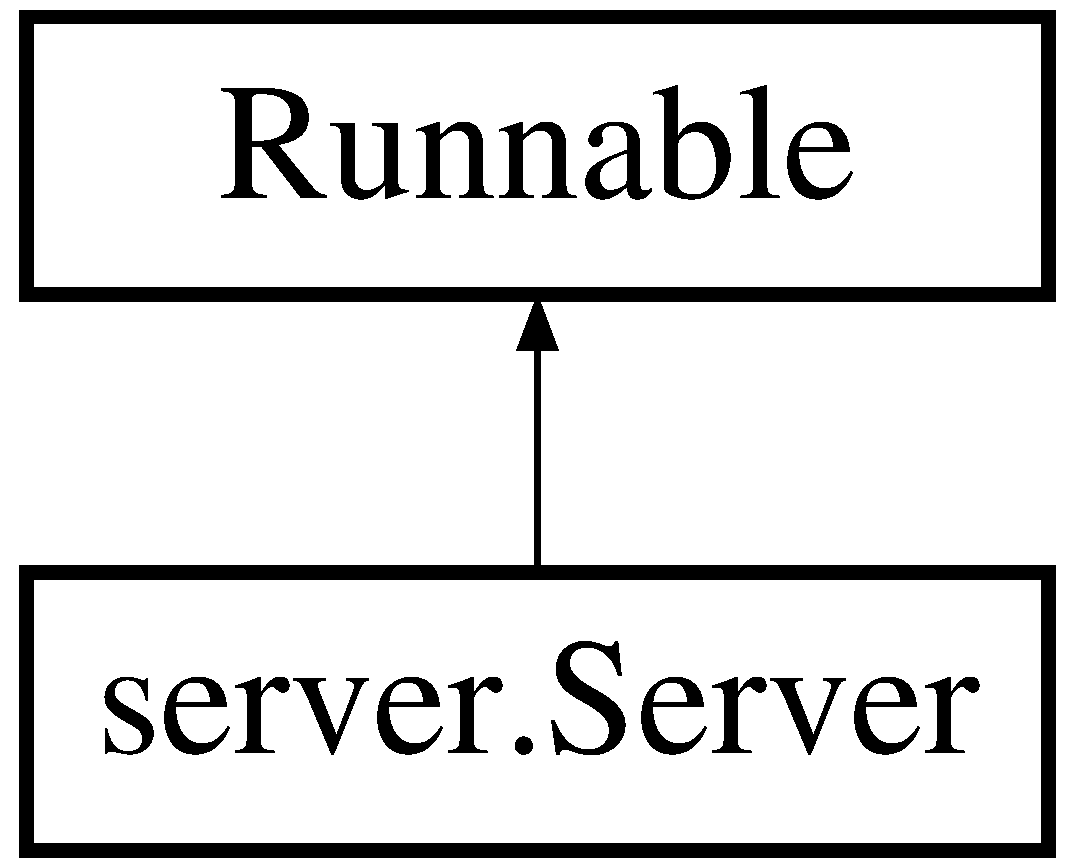
\includegraphics[height=2.000000cm]{classserver_1_1_server}
\end{center}
\end{figure}
\subsection*{Public Member Functions}
\begin{DoxyCompactItemize}
\item 
void \hyperlink{classserver_1_1_server_acd4a76cad17997c1406ef80206a805be}{run} ()
\begin{DoxyCompactList}\small\item\em \hyperlink{classserver_1_1_server}{Server} is waiting for new client connection. \end{DoxyCompactList}\end{DoxyCompactItemize}


\subsection{Detailed Description}


Definition at line 21 of file Server.\+java.



\subsection{Member Function Documentation}
\index{server\+::\+Server@{server\+::\+Server}!run@{run}}
\index{run@{run}!server\+::\+Server@{server\+::\+Server}}
\subsubsection[{\texorpdfstring{run()}{run()}}]{\setlength{\rightskip}{0pt plus 5cm}public void server.\+Server.\+run (
\begin{DoxyParamCaption}
{}
\end{DoxyParamCaption}
)}\hypertarget{classserver_1_1_server_acd4a76cad17997c1406ef80206a805be}{}\label{classserver_1_1_server_acd4a76cad17997c1406ef80206a805be}


\hyperlink{classserver_1_1_server}{Server} is waiting for new client connection. 

\begin{DoxyAuthor}{Author}
Michael Brouchoud 
\end{DoxyAuthor}


Definition at line 108 of file Server.\+java.



The documentation for this class was generated from the following file\+:\begin{DoxyCompactItemize}
\item 
D\+:/owncloud/\+H\+E\+I\+G-\/\+V\+D/\+Java\+Projects/\+G\+E\+N\+\_\+\+Armagetron\+\_\+\+Serveur/src/main/java/server/\hyperlink{_server_8java}{Server.\+java}\end{DoxyCompactItemize}

\hypertarget{classserver_1_1_serveur_tests}{}\section{server.\+Serveur\+Tests Class Reference}
\label{classserver_1_1_serveur_tests}\index{server.\+Serveur\+Tests@{server.\+Serveur\+Tests}}
\subsection*{Public Member Functions}
\begin{DoxyCompactItemize}
\item 
void \hyperlink{classserver_1_1_serveur_tests_ac36116414fd40b3fb27cd7ce615fb026}{test\+Collision} ()  throws Exception
\item 
void \hyperlink{classserver_1_1_serveur_tests_ae4b0b0e8688ab04649b81a0ec471dfa2}{test\+Box\+Collision} ()  throws Exception
\end{DoxyCompactItemize}


\subsection{Detailed Description}


Definition at line 21 of file Serveur\+Tests.\+java.



\subsection{Member Function Documentation}
\index{server\+::\+Serveur\+Tests@{server\+::\+Serveur\+Tests}!test\+Box\+Collision@{test\+Box\+Collision}}
\index{test\+Box\+Collision@{test\+Box\+Collision}!server\+::\+Serveur\+Tests@{server\+::\+Serveur\+Tests}}
\subsubsection[{\texorpdfstring{test\+Box\+Collision()}{testBoxCollision()}}]{\setlength{\rightskip}{0pt plus 5cm}void server.\+Serveur\+Tests.\+test\+Box\+Collision (
\begin{DoxyParamCaption}
{}
\end{DoxyParamCaption}
) throws Exception}\hypertarget{classserver_1_1_serveur_tests_ae4b0b0e8688ab04649b81a0ec471dfa2}{}\label{classserver_1_1_serveur_tests_ae4b0b0e8688ab04649b81a0ec471dfa2}


Definition at line 51 of file Serveur\+Tests.\+java.

\index{server\+::\+Serveur\+Tests@{server\+::\+Serveur\+Tests}!test\+Collision@{test\+Collision}}
\index{test\+Collision@{test\+Collision}!server\+::\+Serveur\+Tests@{server\+::\+Serveur\+Tests}}
\subsubsection[{\texorpdfstring{test\+Collision()}{testCollision()}}]{\setlength{\rightskip}{0pt plus 5cm}void server.\+Serveur\+Tests.\+test\+Collision (
\begin{DoxyParamCaption}
{}
\end{DoxyParamCaption}
) throws Exception}\hypertarget{classserver_1_1_serveur_tests_ac36116414fd40b3fb27cd7ce615fb026}{}\label{classserver_1_1_serveur_tests_ac36116414fd40b3fb27cd7ce615fb026}


Definition at line 24 of file Serveur\+Tests.\+java.



The documentation for this class was generated from the following file\+:\begin{DoxyCompactItemize}
\item 
D\+:/owncloud/\+H\+E\+I\+G-\/\+V\+D/\+Java\+Projects/\+G\+E\+N\+\_\+\+Armagetron\+\_\+\+Serveur/src/test/java/server/\hyperlink{_serveur_tests_8java}{Serveur\+Tests.\+java}\end{DoxyCompactItemize}

\chapter{File Documentation}
\hypertarget{_l_i_c_e_n_s_e_8md}{}\section{D\+:/owncloud/\+H\+E\+I\+G-\/\+V\+D/\+Java\+Projects/\+G\+E\+N\+\_\+\+Armagetron\+\_\+\+Serveur/\+L\+I\+C\+E\+N\+SE.md File Reference}
\label{_l_i_c_e_n_s_e_8md}\index{D\+:/owncloud/\+H\+E\+I\+G-\/\+V\+D/\+Java\+Projects/\+G\+E\+N\+\_\+\+Armagetron\+\_\+\+Serveur/\+L\+I\+C\+E\+N\+S\+E.\+md@{D\+:/owncloud/\+H\+E\+I\+G-\/\+V\+D/\+Java\+Projects/\+G\+E\+N\+\_\+\+Armagetron\+\_\+\+Serveur/\+L\+I\+C\+E\+N\+S\+E.\+md}}

\hypertarget{_client_8java}{}\section{D\+:/owncloud/\+H\+E\+I\+G-\/\+V\+D/\+Java\+Projects/\+G\+E\+N\+\_\+\+Armagetron\+\_\+\+Serveur/src/main/java/client\+Test/\+Client.java File Reference}
\label{_client_8java}\index{D\+:/owncloud/\+H\+E\+I\+G-\/\+V\+D/\+Java\+Projects/\+G\+E\+N\+\_\+\+Armagetron\+\_\+\+Serveur/src/main/java/client\+Test/\+Client.\+java@{D\+:/owncloud/\+H\+E\+I\+G-\/\+V\+D/\+Java\+Projects/\+G\+E\+N\+\_\+\+Armagetron\+\_\+\+Serveur/src/main/java/client\+Test/\+Client.\+java}}
\subsection*{Classes}
\begin{DoxyCompactItemize}
\item 
class \hyperlink{classclient_test_1_1_client}{client\+Test.\+Client}
\end{DoxyCompactItemize}
\subsection*{Packages}
\begin{DoxyCompactItemize}
\item 
package \hyperlink{namespaceclient_test}{client\+Test}
\end{DoxyCompactItemize}

\hypertarget{_box_8java}{}\section{D\+:/owncloud/\+H\+E\+I\+G-\/\+V\+D/\+Java\+Projects/\+G\+E\+N\+\_\+\+Armagetron\+\_\+\+Serveur/src/main/java/server/\+Box.java File Reference}
\label{_box_8java}\index{D\+:/owncloud/\+H\+E\+I\+G-\/\+V\+D/\+Java\+Projects/\+G\+E\+N\+\_\+\+Armagetron\+\_\+\+Serveur/src/main/java/server/\+Box.\+java@{D\+:/owncloud/\+H\+E\+I\+G-\/\+V\+D/\+Java\+Projects/\+G\+E\+N\+\_\+\+Armagetron\+\_\+\+Serveur/src/main/java/server/\+Box.\+java}}


\+: Class Box contained in the Grid\+Game  


\subsection*{Classes}
\begin{DoxyCompactItemize}
\item 
class {\bfseries server.\+Box}
\end{DoxyCompactItemize}
\subsection*{Packages}
\begin{DoxyCompactItemize}
\item 
package \hyperlink{namespaceserver}{server}
\end{DoxyCompactItemize}


\subsection{Detailed Description}
\+: Class Box contained in the Grid\+Game 

\+: Argmagetron

\begin{DoxyAuthor}{Author}
(s) \+: Thomas Lechaire 
\end{DoxyAuthor}
\begin{DoxyDate}{Date}
\+: 11.\+05.\+2017 
\end{DoxyDate}

\hypertarget{_client_thread_8java}{}\section{D\+:/owncloud/\+H\+E\+I\+G-\/\+V\+D/\+Java\+Projects/\+G\+E\+N\+\_\+\+Armagetron\+\_\+\+Serveur/src/main/java/server/\+Client\+Thread.java File Reference}
\label{_client_thread_8java}\index{D\+:/owncloud/\+H\+E\+I\+G-\/\+V\+D/\+Java\+Projects/\+G\+E\+N\+\_\+\+Armagetron\+\_\+\+Serveur/src/main/java/server/\+Client\+Thread.\+java@{D\+:/owncloud/\+H\+E\+I\+G-\/\+V\+D/\+Java\+Projects/\+G\+E\+N\+\_\+\+Armagetron\+\_\+\+Serveur/src/main/java/server/\+Client\+Thread.\+java}}


\+: Use as interface between client and controller to receive object from server, send object to server and connect to the server  


\subsection*{Classes}
\begin{DoxyCompactItemize}
\item 
class {\bfseries server.\+Client\+Thread}
\end{DoxyCompactItemize}
\subsection*{Packages}
\begin{DoxyCompactItemize}
\item 
package \hyperlink{namespaceserver}{server}
\end{DoxyCompactItemize}


\subsection{Detailed Description}
\+: Use as interface between client and controller to receive object from server, send object to server and connect to the server 

\+: Argmagetron

\begin{DoxyAuthor}{Author}
(s) \+: Michael Brouchoud 
\end{DoxyAuthor}
\begin{DoxyDate}{Date}
\+: 18.\+05.\+2017 
\end{DoxyDate}

\hypertarget{_controller_8java}{}\section{D\+:/owncloud/\+H\+E\+I\+G-\/\+V\+D/\+Java\+Projects/\+G\+E\+N\+\_\+\+Armagetron\+\_\+\+Serveur/src/main/java/server/\+Controller.java File Reference}
\label{_controller_8java}\index{D\+:/owncloud/\+H\+E\+I\+G-\/\+V\+D/\+Java\+Projects/\+G\+E\+N\+\_\+\+Armagetron\+\_\+\+Serveur/src/main/java/server/\+Controller.\+java@{D\+:/owncloud/\+H\+E\+I\+G-\/\+V\+D/\+Java\+Projects/\+G\+E\+N\+\_\+\+Armagetron\+\_\+\+Serveur/src/main/java/server/\+Controller.\+java}}


\+: Check all data between Game and Server  


\subsection*{Classes}
\begin{DoxyCompactItemize}
\item 
class {\bfseries server.\+Controller}
\end{DoxyCompactItemize}
\subsection*{Packages}
\begin{DoxyCompactItemize}
\item 
package \hyperlink{namespaceserver}{server}
\end{DoxyCompactItemize}


\subsection{Detailed Description}
\+: Check all data between Game and Server 

\+: Argmagetron

\begin{DoxyAuthor}{Author}
(s) \+: Michael Brouchoud 
\end{DoxyAuthor}
\begin{DoxyDate}{Date}
\+: 30.\+05.\+2017 
\end{DoxyDate}

\hypertarget{_game_8java}{}\section{D\+:/owncloud/\+H\+E\+I\+G-\/\+V\+D/\+Java\+Projects/\+G\+E\+N\+\_\+\+Armagetron\+\_\+\+Serveur/src/main/java/server/\+Game.java File Reference}
\label{_game_8java}\index{D\+:/owncloud/\+H\+E\+I\+G-\/\+V\+D/\+Java\+Projects/\+G\+E\+N\+\_\+\+Armagetron\+\_\+\+Serveur/src/main/java/server/\+Game.\+java@{D\+:/owncloud/\+H\+E\+I\+G-\/\+V\+D/\+Java\+Projects/\+G\+E\+N\+\_\+\+Armagetron\+\_\+\+Serveur/src/main/java/server/\+Game.\+java}}


\+: Use only for the Tests  


\subsection*{Classes}
\begin{DoxyCompactItemize}
\item 
class {\bfseries server.\+Game}
\end{DoxyCompactItemize}
\subsection*{Packages}
\begin{DoxyCompactItemize}
\item 
package \hyperlink{namespaceserver}{server}
\end{DoxyCompactItemize}


\subsection{Detailed Description}
\+: Use only for the Tests 

\+: Use to Manage the Game

\+: Argmagetron

\begin{DoxyAuthor}{Author}
(s) \+: Michael Brouchoud 
\end{DoxyAuthor}
\begin{DoxyDate}{Date}
\+: 30.\+05.\+2017 
\end{DoxyDate}

\hypertarget{_game_grid_8java}{}\section{D\+:/owncloud/\+H\+E\+I\+G-\/\+V\+D/\+Java\+Projects/\+G\+E\+N\+\_\+\+Armagetron\+\_\+\+Serveur/src/main/java/server/\+Game\+Grid.java File Reference}
\label{_game_grid_8java}\index{D\+:/owncloud/\+H\+E\+I\+G-\/\+V\+D/\+Java\+Projects/\+G\+E\+N\+\_\+\+Armagetron\+\_\+\+Serveur/src/main/java/server/\+Game\+Grid.\+java@{D\+:/owncloud/\+H\+E\+I\+G-\/\+V\+D/\+Java\+Projects/\+G\+E\+N\+\_\+\+Armagetron\+\_\+\+Serveur/src/main/java/server/\+Game\+Grid.\+java}}


\+: class use to manage the Game\+Grid  


\subsection*{Classes}
\begin{DoxyCompactItemize}
\item 
class {\bfseries server.\+Game\+Grid}
\end{DoxyCompactItemize}
\subsection*{Packages}
\begin{DoxyCompactItemize}
\item 
package \hyperlink{namespaceserver}{server}
\end{DoxyCompactItemize}


\subsection{Detailed Description}
\+: class use to manage the Game\+Grid 

\+: Argmagetron

\begin{DoxyAuthor}{Author}
(s) \+: Thomas Lechaire 
\end{DoxyAuthor}
\begin{DoxyDate}{Date}
\+: 11.\+05.\+2017 
\end{DoxyDate}

\hypertarget{_location_8java}{}\section{D\+:/owncloud/\+H\+E\+I\+G-\/\+V\+D/\+Java\+Projects/\+G\+E\+N\+\_\+\+Armagetron\+\_\+\+Serveur/src/main/java/server/\+Location.java File Reference}
\label{_location_8java}\index{D\+:/owncloud/\+H\+E\+I\+G-\/\+V\+D/\+Java\+Projects/\+G\+E\+N\+\_\+\+Armagetron\+\_\+\+Serveur/src/main/java/server/\+Location.\+java@{D\+:/owncloud/\+H\+E\+I\+G-\/\+V\+D/\+Java\+Projects/\+G\+E\+N\+\_\+\+Armagetron\+\_\+\+Serveur/src/main/java/server/\+Location.\+java}}


\+: Class Location use to set Starting location to player  


\subsection*{Classes}
\begin{DoxyCompactItemize}
\item 
class \hyperlink{classserver_1_1_location}{server.\+Location}
\end{DoxyCompactItemize}
\subsection*{Packages}
\begin{DoxyCompactItemize}
\item 
package \hyperlink{namespaceserver}{server}
\end{DoxyCompactItemize}


\subsection{Detailed Description}
\+: Class Location use to set Starting location to player 

\+: Argmagetron

\begin{DoxyAuthor}{Author}
(s) \+: Thomas Lechaire 
\end{DoxyAuthor}
\begin{DoxyDate}{Date}
\+: 11.\+05.\+2017 
\end{DoxyDate}

\hypertarget{_main_8java}{}\section{D\+:/owncloud/\+H\+E\+I\+G-\/\+V\+D/\+Java\+Projects/\+G\+E\+N\+\_\+\+Armagetron\+\_\+\+Serveur/src/main/java/server/\+Main.java File Reference}
\label{_main_8java}\index{D\+:/owncloud/\+H\+E\+I\+G-\/\+V\+D/\+Java\+Projects/\+G\+E\+N\+\_\+\+Armagetron\+\_\+\+Serveur/src/main/java/server/\+Main.\+java@{D\+:/owncloud/\+H\+E\+I\+G-\/\+V\+D/\+Java\+Projects/\+G\+E\+N\+\_\+\+Armagetron\+\_\+\+Serveur/src/main/java/server/\+Main.\+java}}


\+: Start a new server  


\subsection*{Classes}
\begin{DoxyCompactItemize}
\item 
class \hyperlink{classserver_1_1_main}{server.\+Main}
\end{DoxyCompactItemize}
\subsection*{Packages}
\begin{DoxyCompactItemize}
\item 
package \hyperlink{namespaceserver}{server}
\end{DoxyCompactItemize}


\subsection{Detailed Description}
\+: Start a new server 

\+: Argmagetron

\begin{DoxyAuthor}{Author}
(s) \+: Michael Brouchoud 
\end{DoxyAuthor}
\begin{DoxyDate}{Date}
\+: 30.\+05.\+2017 
\end{DoxyDate}

\hypertarget{_player_8java}{}\section{D\+:/owncloud/\+H\+E\+I\+G-\/\+V\+D/\+Java\+Projects/\+G\+E\+N\+\_\+\+Armagetron\+\_\+\+Serveur/src/main/java/server/\+Player.java File Reference}
\label{_player_8java}\index{D\+:/owncloud/\+H\+E\+I\+G-\/\+V\+D/\+Java\+Projects/\+G\+E\+N\+\_\+\+Armagetron\+\_\+\+Serveur/src/main/java/server/\+Player.\+java@{D\+:/owncloud/\+H\+E\+I\+G-\/\+V\+D/\+Java\+Projects/\+G\+E\+N\+\_\+\+Armagetron\+\_\+\+Serveur/src/main/java/server/\+Player.\+java}}


\+: Use to manage a player  


\subsection*{Classes}
\begin{DoxyCompactItemize}
\item 
class {\bfseries server.\+Player}
\end{DoxyCompactItemize}
\subsection*{Packages}
\begin{DoxyCompactItemize}
\item 
package \hyperlink{namespaceserver}{server}
\end{DoxyCompactItemize}


\subsection{Detailed Description}
\+: Use to manage a player 

\+: Argmagetron

\begin{DoxyAuthor}{Author}
(s) \+: Michael Brouchoud 
\end{DoxyAuthor}
\begin{DoxyDate}{Date}
\+: 18.\+05.\+2017 
\end{DoxyDate}

\hypertarget{_server_8java}{}\section{D\+:/owncloud/\+H\+E\+I\+G-\/\+V\+D/\+Java\+Projects/\+G\+E\+N\+\_\+\+Armagetron\+\_\+\+Serveur/src/main/java/server/\+Server.java File Reference}
\label{_server_8java}\index{D\+:/owncloud/\+H\+E\+I\+G-\/\+V\+D/\+Java\+Projects/\+G\+E\+N\+\_\+\+Armagetron\+\_\+\+Serveur/src/main/java/server/\+Server.\+java@{D\+:/owncloud/\+H\+E\+I\+G-\/\+V\+D/\+Java\+Projects/\+G\+E\+N\+\_\+\+Armagetron\+\_\+\+Serveur/src/main/java/server/\+Server.\+java}}


\+: Server  


\subsection*{Classes}
\begin{DoxyCompactItemize}
\item 
class \hyperlink{classserver_1_1_server}{server.\+Server}
\end{DoxyCompactItemize}
\subsection*{Packages}
\begin{DoxyCompactItemize}
\item 
package \hyperlink{namespaceserver}{server}
\end{DoxyCompactItemize}


\subsection{Detailed Description}
\+: Server 

\+: Argmagetron

\begin{DoxyAuthor}{Author}
(s) \+: Michael Brouchoud 
\end{DoxyAuthor}
\begin{DoxyDate}{Date}
\+: 18.\+05.\+2017 
\end{DoxyDate}

\hypertarget{_box_test_8java}{}\section{D\+:/owncloud/\+H\+E\+I\+G-\/\+V\+D/\+Java\+Projects/\+G\+E\+N\+\_\+\+Armagetron\+\_\+\+Serveur/src/test/java/server/\+Box\+Test.java File Reference}
\label{_box_test_8java}\index{D\+:/owncloud/\+H\+E\+I\+G-\/\+V\+D/\+Java\+Projects/\+G\+E\+N\+\_\+\+Armagetron\+\_\+\+Serveur/src/test/java/server/\+Box\+Test.\+java@{D\+:/owncloud/\+H\+E\+I\+G-\/\+V\+D/\+Java\+Projects/\+G\+E\+N\+\_\+\+Armagetron\+\_\+\+Serveur/src/test/java/server/\+Box\+Test.\+java}}


\+: Test the class Box  


\subsection*{Classes}
\begin{DoxyCompactItemize}
\item 
class \hyperlink{classserver_1_1_box_test}{server.\+Box\+Test}
\end{DoxyCompactItemize}
\subsection*{Packages}
\begin{DoxyCompactItemize}
\item 
package \hyperlink{namespaceserver}{server}
\end{DoxyCompactItemize}


\subsection{Detailed Description}
\+: Test the class Box 

\+: Argmagetron

\begin{DoxyAuthor}{Author}
(s) \+: Michaël Brouchoud 
\end{DoxyAuthor}
\begin{DoxyDate}{Date}
\+: 18.\+05.\+2017 
\end{DoxyDate}

\hypertarget{_controller_test_8java}{}\section{D\+:/owncloud/\+H\+E\+I\+G-\/\+V\+D/\+Java\+Projects/\+G\+E\+N\+\_\+\+Armagetron\+\_\+\+Serveur/src/test/java/server/\+Controller\+Test.java File Reference}
\label{_controller_test_8java}\index{D\+:/owncloud/\+H\+E\+I\+G-\/\+V\+D/\+Java\+Projects/\+G\+E\+N\+\_\+\+Armagetron\+\_\+\+Serveur/src/test/java/server/\+Controller\+Test.\+java@{D\+:/owncloud/\+H\+E\+I\+G-\/\+V\+D/\+Java\+Projects/\+G\+E\+N\+\_\+\+Armagetron\+\_\+\+Serveur/src/test/java/server/\+Controller\+Test.\+java}}


\+: Test the class Controller\+Test  


\subsection*{Classes}
\begin{DoxyCompactItemize}
\item 
class \hyperlink{classserver_1_1_controller_test}{server.\+Controller\+Test}
\end{DoxyCompactItemize}
\subsection*{Packages}
\begin{DoxyCompactItemize}
\item 
package \hyperlink{namespaceserver}{server}
\end{DoxyCompactItemize}


\subsection{Detailed Description}
\+: Test the class Controller\+Test 

\+: Argmagetron

\begin{DoxyAuthor}{Author}
(s) \+: Michaël Brouchoud 
\end{DoxyAuthor}
\begin{DoxyDate}{Date}
\+: 05.\+06.\+2017 
\end{DoxyDate}

\hypertarget{_game_test_8java}{}\section{D\+:/owncloud/\+H\+E\+I\+G-\/\+V\+D/\+Java\+Projects/\+G\+E\+N\+\_\+\+Armagetron\+\_\+\+Serveur/src/test/java/server/\+Game\+Test.java File Reference}
\label{_game_test_8java}\index{D\+:/owncloud/\+H\+E\+I\+G-\/\+V\+D/\+Java\+Projects/\+G\+E\+N\+\_\+\+Armagetron\+\_\+\+Serveur/src/test/java/server/\+Game\+Test.\+java@{D\+:/owncloud/\+H\+E\+I\+G-\/\+V\+D/\+Java\+Projects/\+G\+E\+N\+\_\+\+Armagetron\+\_\+\+Serveur/src/test/java/server/\+Game\+Test.\+java}}
\subsection*{Classes}
\begin{DoxyCompactItemize}
\item 
class \hyperlink{classserver_1_1_game_test}{server.\+Game\+Test}
\end{DoxyCompactItemize}
\subsection*{Packages}
\begin{DoxyCompactItemize}
\item 
package \hyperlink{namespaceserver}{server}
\end{DoxyCompactItemize}

\hypertarget{_serveur_tests_8java}{}\section{D\+:/owncloud/\+H\+E\+I\+G-\/\+V\+D/\+Java\+Projects/\+G\+E\+N\+\_\+\+Armagetron\+\_\+\+Serveur/src/test/java/server/\+Serveur\+Tests.java File Reference}
\label{_serveur_tests_8java}\index{D\+:/owncloud/\+H\+E\+I\+G-\/\+V\+D/\+Java\+Projects/\+G\+E\+N\+\_\+\+Armagetron\+\_\+\+Serveur/src/test/java/server/\+Serveur\+Tests.\+java@{D\+:/owncloud/\+H\+E\+I\+G-\/\+V\+D/\+Java\+Projects/\+G\+E\+N\+\_\+\+Armagetron\+\_\+\+Serveur/src/test/java/server/\+Serveur\+Tests.\+java}}


\+: Class vérifiant les collisions sur le serveur  


\subsection*{Classes}
\begin{DoxyCompactItemize}
\item 
class \hyperlink{classserver_1_1_serveur_tests}{server.\+Serveur\+Tests}
\end{DoxyCompactItemize}
\subsection*{Packages}
\begin{DoxyCompactItemize}
\item 
package \hyperlink{namespaceserver}{server}
\end{DoxyCompactItemize}


\subsection{Detailed Description}
\+: Class vérifiant les collisions sur le serveur 

\+: Argmagetron

\begin{DoxyAuthor}{Author}
(s) \+: Thomas Léchaire 
\end{DoxyAuthor}
\begin{DoxyDate}{Date}
\+: 01.\+06.\+2017 
\end{DoxyDate}

\hypertarget{_test_utils_8java}{}\section{D\+:/owncloud/\+H\+E\+I\+G-\/\+V\+D/\+Java\+Projects/\+G\+E\+N\+\_\+\+Armagetron\+\_\+\+Serveur/src/test/java/server/\+Test\+Utils.java File Reference}
\label{_test_utils_8java}\index{D\+:/owncloud/\+H\+E\+I\+G-\/\+V\+D/\+Java\+Projects/\+G\+E\+N\+\_\+\+Armagetron\+\_\+\+Serveur/src/test/java/server/\+Test\+Utils.\+java@{D\+:/owncloud/\+H\+E\+I\+G-\/\+V\+D/\+Java\+Projects/\+G\+E\+N\+\_\+\+Armagetron\+\_\+\+Serveur/src/test/java/server/\+Test\+Utils.\+java}}


\+: Utils Object shared by Test class  


\subsection*{Classes}
\begin{DoxyCompactItemize}
\item 
class {\bfseries server.\+Test\+Utils}
\end{DoxyCompactItemize}
\subsection*{Packages}
\begin{DoxyCompactItemize}
\item 
package \hyperlink{namespaceserver}{server}
\end{DoxyCompactItemize}


\subsection{Detailed Description}
\+: Utils Object shared by Test class 

\+: Argmagetron

\begin{DoxyAuthor}{Author}
(s) \+: Michaël Brouchoud 
\end{DoxyAuthor}
\begin{DoxyDate}{Date}
\+: 30.\+05.\+2017 
\end{DoxyDate}

%--- End generated contents ---

% Index
\backmatter
\newpage
\phantomsection
\clearemptydoublepage
\addcontentsline{toc}{chapter}{Index}
\printindex

\end{document}
